\chapter{Vergleich AOT vs. JIT}

\section{Programmausführung in der VM} \label{jit_vm}
Durch die Dynamik einer Programmiersprache, zur Schaffung einer Plattformunabhängigkeit oder aus Sicherheitsgründen werden Programme heutzutage oftmals nicht mehr direkt vom Betriebssystem ausgeführt, sondern laufen in einer \ac{VM}, wie dies bereits bei Smaltalk-80 der Fall war. Dies verzögert jedoch die Ausführungszeit der Interpretation der Befehle. \\
Durch die Anwendung von \ac{JIT} wird hier versucht Performance zu gewinnen und somit diesen Nachteil auszugleichen. Folgend sollen die beiden \ac{VM}'s 'HotSpot' und 'GraalVM' aus dem Kontext der Sprache Java näher vorgestellt werden. 

\subsection{HotSpot}
Java übersetzt den Code der Hochsprache generell zuerst in Bytecode, der in der \ac{VM} ausgeführt werden kann. Diese \ac{VM} wird speziell für das korrespondierende \ac{OS} bereitgestellt und kann auf dieser Plattform den erzeugten Bytecode korrekt ausführen. 'HotSpot' von Oracle ist eine dieser \ac{VM}'s für die Sprache Java. \\
\\
\begin{figure}[ht]
    \begin{center}
        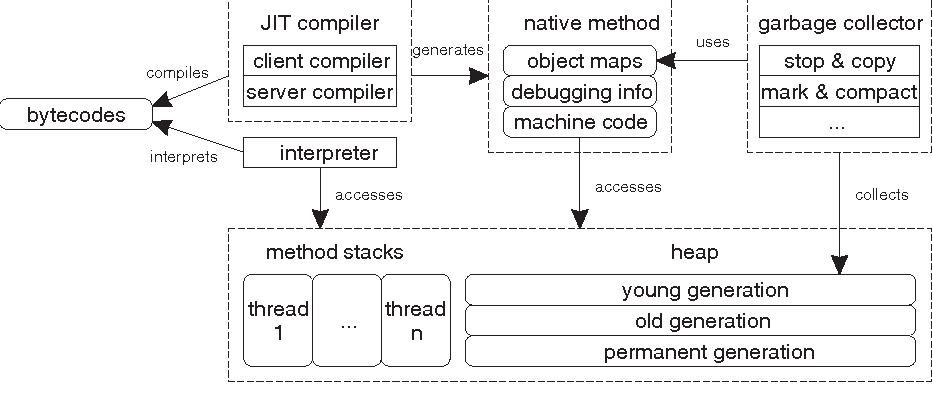
\includegraphics[width=0.9\textwidth]{assets/img/3-Figure1-1.png}
        \caption{Architektur 'HotSpot', \cite[Quelle: Kotzmann Wimmer 2008]{KotzmannWimmer2008}}
        \label{arch_hotspot}
    \end{center}
\end{figure}
Wie in \autoref{arch_hotspot} zu sehen, beginnt die Ausführung in der 'HotSpot'-\ac{VM} beim Interpreter. Hier wird der Bytecode schrittweise anhand von Templates ausgeführt. Nur die heuristisch am meisten frequentierten Codeblöcke werden durch den \ac{JIT}-Compiler kompiliert.\\
Wird während der Ausführung eine besonders aufwändige Schleife entdeckt, so wird diese ebenfalls kompiliert und die Ausführung dafür gestoppt. Die Schwierigkeit besteht hierbei darin, dass die Ausführung zwischen Interpreter und dem kompilierten Code synchronisiert werden muss. Dafür wird ein neuer Stackframe erstellt und initialisiert. Die Ausführung der Methode geht im nativen Code weiter. Dieses Verfahren nennt man \ac{OSR}.\\
'HotSpot' enthält zwei verschiedene Compiler, die für Server- und Clientsysteme gedacht sind. Bei Serversystemen wird sehr großer Wert auf eine sehr gute Optimierung gelegt, dafür jedoch eine längere Kompilierungszeit in Kauf genommen. Für dauerhaft laufende Serveranwendungen geht man davon aus, dass bereits während der Anlaufphase der Software der \ac{JIT}-Compiler alle wichtigen Methoden und Blöcke kompiliert und optimiert. Die längere Zeit ist hierfür nicht relevant, da die einmal kompilierten Sequenzen danach während der ganzen Laufzeit der Software zu Verfügung stehen.\\
Der Compiler für die Clientsysteme zielt auf Programme mit \ac{GUI} ab. Hier wird der Fokus auf die Antwortzeit der Oberfläche und damit den Punkt \ac{UX} gelegt. Dazu ist der \ac{JIT}-Compiler auf eine schnelle Kompilierung statt Performance ausgelegt.\\
Reservierter Speicher wird in drei Bereichen verwaltet. Neu kompilierte Methoden werden zuerst im Bereich der 'Young Generation' abgelegt. Füllt sich dieser Bereich, wird eine 'stop-and-copy' \ac{GC} initialisiert. Diese prüft, ob ein Objekt noch in Benutzung ist und löscht alle übrigen, um Speicher wieder freizugeben. Übersteht eine Methode mehrere Runden, wird sie in den Bereich der 'Old Generation' übernommen. Der Dritte Bereich wird als 'Permanent Generation' bezeichnet und enthält interne Datenstrukturen. Dieses Schema ist in \autoref{arch_hotspot} dargestellt, \cite[vgl. Kotzmann und Wimmer 2008, S.3f]{KotzmannWimmer2008}.\\

\subsubsection{Optimierung/Profiling}
Wie bereits erwähnt versucht der \ac{JIT}-Compiler durch Spekulationen und Heuristik die Performance in der Ausführung des Codes zu erhöhen. Da es sich bei dieser Optimierung nicht um eine Methode des Prinzips des 'Trial and Error' handelt müssen getätigte Optimierung auch wieder rückgängig gemacht werden können (Deoptimierung).\\
Mit Profildaten, die während der Ausführung gesammelt werden und Aufschluss über den Ablauf des Programmes geben, wird weiterhin versucht, die Optimierung gezielter auf Basis von Daten anzugehen und hierdurch Optimierungs-Entscheidungen rationaler und weniger spekulativ zu treffen. Dadurch sollen Deoptimierungsvorgänge so stark wie möglich reduziert werden und damit Ressourcen und Performance eingespart werden.\\
Der \ac{JIT}-Compiler arbeitet mit Ebenen, wobei man grundsätzlich  in High und Low unterscheiden kann. Die sogenannten 'Hot Spots', also Methoden, die sehr oft ausgeführt werden und damit am meisten von einer Optimierung profitieren werden dabei in die High-Ebene eingeordnet. Code, der nur mittels des Interpreters oder ein schwach Optimierten Kompilierung ausgeführt wird, ordnet man die Low-Ebene ein. Da das Optimieren und Kompilieren sehr viele Ressourcen benötigt, kann nicht der ganze Code optimiert werden und die Optimierung wird auf die 'Hot Spots' fokussiert.\\
Das Profiling setzt nun hier an und sammelt Informationen während der Laufzeit, um eine Optimierung eines potenziellen HotSpots zu rechtfertigen. Code wird ausgeführt und getrackt. Mittels von Zählern können HotSpots erkannt und diese der High-Ebene mit hohem Optimierungsgrad zugeordnet werden. Das Ziel ist es hierbei, dass Hot-Spots schon sehr früh während der Ausführung erkannt werden und somit alle kritischen Methoden mit höchstmöglicher Optimierung laufen, um der Anwendung eine bestmögliche Performance zu geben. Die Methoden der Low-Ebene sind unkritisch, da sie nur einen geringen Teil zur Laufzeit beitragen. \\
Durch die ständige Überwachung und Sammlung von Daten kann der Compiler bei der Hochstufung einer Methode von der Low- in die Highebene auf die zuvor gesammelten Datenpunkte zurückgreifen und damit die Spekulationen zur Optimierung steuern und rationalisieren. Das Profiling in der Low-Ebene kostet zwar wiederum Ressourcen und Performance, aber fällt nicht ins Gewicht, da diese Methoden nicht hoch frequentiert sind. Der Nutzen von gesammelten Daten wiederum zahlt sich wiederum aus, wenn die betreffende Methode hochgestuft und optimiert wird. Das macht die Applikation im Ganzen wesentlich performanter.\\
\\
Profilbasierte Optimierungen sind nicht unbedingt an \ac{JIT}-Compiler gebunden, sondern können auch im Bereich der \ac{AOT} Anwendung finden. Statt zu Laufzeit wird hier im Vorfeld durch Trainingsläufe optimiert. Im Gegensatz zur Optimierung im \ac{JIT}-Sektor ist hier also ein Mehraufwand für die Entwickler gegeben, \cite[vgl. Westrelin 2021, Webseite abgerufen am 02.12.2022]{westrelin_2022}



\subsection{GraalVM }
Die GraalVM ("General Recursive Applicative and Algorithmic Language Virtual Machine")  ist ein System, das die \ac{VM} HotSpot ergänzen soll und dazu ein breites Subsystem an Tools für mehr Flexibilität mitbringt (siehe \autoref{arch_graal}). GraalVM zeichnet sich dadurch aus, dass es komplett selbst in Java geschrieben ist. \\
\\
\begin{figure}[ht]
    \begin{center}
        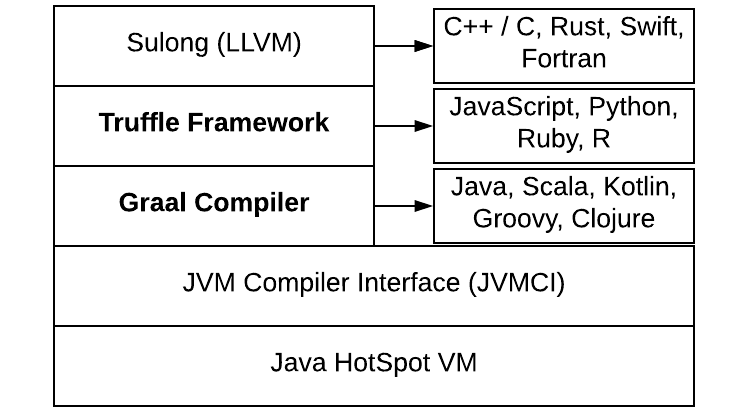
\includegraphics[width=0.9\textwidth]{assets/img/GraalVM-Architecture.png}
        \caption{Architektur 'GraalVM ', \cite[Quelle: Sipek 2020]{Sipek_2020}}
        \label{arch_graal}
    \end{center}
\end{figure}
GraalVM  setzt an der HotSpot \ac{VM} an und nutzt alle HotSpot Komponenten, die nicht direkt in den Prozess der Kompilierung eingebunden sind. Diese Kompilierungstools stellt GraalVM selbst zur Verfügung und wird über die \ac{JVMCI} mit der HotSpot \ac{VM} verbunden. \\
Die Motivation für den Tausch des Compilers oberhalb der \ac{VM} liegt in dessen Vielfältigkeit. Wie in \autoref{arch_graal} zu sehen bringt der Graal-Compiler ein breites Subsystem mit, dass eine Anwendung sehr viel flexibler machen kann. Der integrierte GraalVM Compiler unterstützt \ac{JVM} basierte Sprachen, wie Java, Scala, Kotlin, Groovy oder Clojure und kann somit als generalisierter \ac{JIT} Compiler für eine breite Plattform an Sprachen eingesetzt werden. Dies macht es für Entwickler wesentlich einfacher in den genannten Sprachen zu entwickeln, wenn sie bereits mit der zugrunde liegenden Technik von HotSpot vertraut sind. Ein Wechsel des Technik-Stacks entfällt und ein Einstieg in neue Sprachen fällt ungemein leichter. \\
Neben der Funktion als \ac{JIT}-Compiler bringt GraalVM auch die Möglichkeit mit, native Images zu erstellen und somit den Ansatz des \ac{AOT} zu erfüllen. Dieses Feature wird in \autoref{graal_aot} näher beleuchtet.\\
Das in \autoref{arch_graal} noch ersichtliche Truffle-Framework führt einen ähnlichen Ansatz, wie bereits der in GraalVM integrierte Compiler und erweitert die \ac{VM} für den Support weiterer Sprachen, wie z.B. JavaScript, Python, Ruby oder R. Truffle nutzt einen \ac{AST}, um den Code zu interpretieren und auszuführen. Dies stellt einen sehr einfachen Weg dar, kostet aber Ressourcen und kann z.T. in einer schwachen Performance resultieren. GraalVM setzt hier an und kann erzeugte \ac{AST} in hochoptimierte native ausführbare Dateien kompilieren. Um Overhead einzusparen kann dabei eine beliebige Anzahl \ac{AST} verbunden werden und als ein einziger interpretiert werden.\\
Über Truffle steht noch die Compiler-Infrastruktur-Engine 'Sulong', die Bitcode aus Low-Level Sprachen, wie z.B. C, C++, Fortan, Rust oder Swift, interpretieren kann. Das erweitert das Einsatzspektrum der GraalVM  nochmals stark und es kann nahezu das ganze Feld der bekannten Sprachen eingesetzt werden \cite[vgl. Sipek 2020, S.2]{Sipek_2020}.\\

\subsubsection{Native Image: GraalVM als AOT-Compiler} \label{graal_aot}
Wie bereits beschrieben verfügt die GraalVM neben einem \ac{JIT}-Compiler auch über einen \ac{AOT}-Compiler, der ein Programm statt in Bytecode direkt in ein natives Image kompiliert.\\
\\
\begin{figure}[ht]
    \begin{center}
        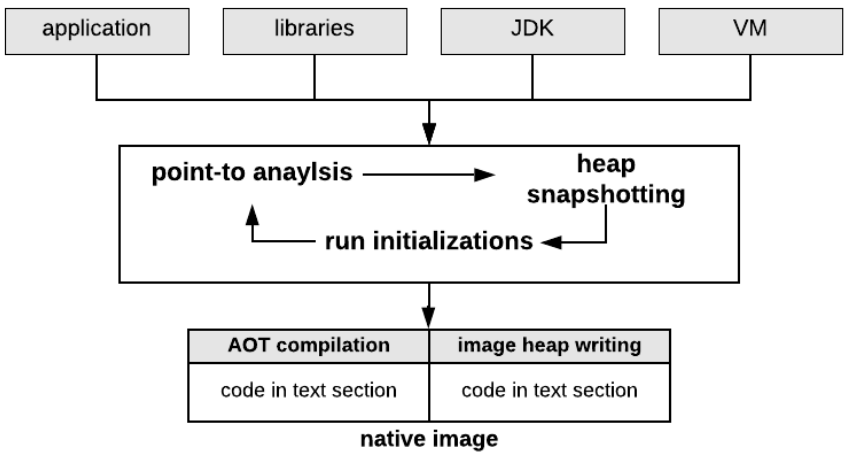
\includegraphics[width=0.9\textwidth]{assets/img/graal_nativeimg.PNG}
        \caption{GraalVM Native Image Erzeugung, \cite[Quelle: Sipek 2020]{Sipek_2020}}
        \label{graal_nativeimg}
    \end{center}
\end{figure}
Wie in \autoref{graal_nativeimg} zu sehen wird dabei in mehreren Schritten vorgegangen, um von der Hochsprache bis zu einem Image zu kommen, das sowohl den Code, als auch alle genutzten Bibliotheken, das genutzte \ac{JDK} und die zugrundeliegende VM vereint und damit alles, was zur Ausführung auf dem Zielsystem benötigt wird, in einer einzigen Datei bündelt.\\
In einer 'point-to-Analyse' wird die Ausführung des Programms iterativ immer wieder bis zu bestimmten Punkten durchgespielt und bei Erreichen des genannten Punktes angehalten. Alle Programmteile, die während dieses teilweisen Durchlaufes erreicht werden, werden getrackt und alle benötigten Teile dieser Klassen, inkl. Felder und Methoden, sowie der genutzten Teile der eingebundenen Bibliotheken eingebunden. Während dieser 'point-to-Analyse' wird durch den Graal-Compiler Java Bytecode in \ac{Graal IR} gewandelt.\\
Alle getrackten Codeblöcke werden danach initialisiert und aus allen hierbei erzeugten Objekte durch den 'heap-snaphotting'-Mechanismus ein Objektgraph erzeugt. \\
Das ganze Verfahren aus 'point-to-Analyse', Initialisierung und 'heap-snapshotting' wird iterativ so oft durchgeführt, bis keine Änderungen zur vorherigen Iteration mehr festgestellt werden können. Es wird nun davon ausgegangen, dass der komplette Programmablauf einmal durchgespielt wurde und alle benötigten Daten für das Image gesammelt sind.\\
Der erstandene Objektgraph wird als 'image-heap' angenommen und alle darin entstandenen Objekte werden serialisiert und in eine Sektion im Image eingebaut. \\
\\
Der Compiler, der bei diesem Vorgang der \ac{AOT}-Kompilierung genutzt wird unterscheidet sich zu dem ebenfalls in GraalVM enthaltenen \ac{JIT}-Compiler insofern, als, dass bei der \ac{AOT}-Kompilierung keine Deoptimierungen gemacht werden können, die mit der spekulativen Optimierung des \ac{JIT}-Compilers zwingend einhergehen. Hier wird daher aufgrund von Ergebnissen aus der 'point-to-Analyse' optimiert. Der image-heap wird aus mehreren Schichten (Stacks) gebildet, was in einem ausführbaren Image mit vorherbestimmten Heap-Speicher resultiert, \cite[vgl. Sipek 2020, S.3]{Sipek_2020}.

\subsection{HotSpot vs Graal}

\section{Anwendungsgebiete}
Für sowohl \ac{AOT}, als auch \ac{JIT} gibt es Anwendungsgebiete, in denen sie ihre Vorteile stark ausspielen können. Folgend sollen einige grundlegende Szenarien dargelegt werden und anschließend auch auf einige direkte Beispiele eingegangen werden. 

\subsection{AOT}
Es gibt viele Bereiche, in denen die Implementierungsform der \ac{AOT}-Kompilierung unerlässlich ist. Gerade auf Leistungsschwachen Plattformen kann durch schlanke Applikationen in C, die zu einer nativen Applikation kompiliert werden, eine sehr gute Performance erreicht werden. Dies gilt z.B. für embedded-Geräte und auch Mikrocontroller im Bereich der Steuerungstechnik. Auf diesen Plattformen sind Ressourcen, wie Rechenpower und Arbeitsspeicher meist teuer und deshalb stark begrenzt. Der Einsatz eines \ac{JIT}-Compilers mit großem Overhead ist daher nicht möglich oder nicht zu empfehlen. Die Hardware ist hier bereits im Vorfeld ganz genau bekannt und es kann explizit für genau dieses Setting kompiliert und optimiert werden. Das Set an Maschinenbefehlen, die das Zielsystem unterstützt, ist bekannt und kann optimal ausgenutzt werden, um eine bestmögliche Performance zu erhalten. \\
Solche Systeme werden außerdem nicht so oft mit Updates versorgt und die Dauer der Kompilierung für eine native Applikation spielt hier so keine größere Rolle. Die Funktion der Software ist einfach gehalten und einmal aufgespielt können sehr viele Zyklen durchlaufen werden, die alle immer gleich schnell ausgeführt werden. Da es sich außerdem z.T. um sicherheitskritische Software handelt, soll diese zur Laufzeit nicht veränderbar sein. Nach der Kompilierung kann die Software auch ein Auditverfaren durchlaufen, um geprüft und freigegeben werden zu können. Hier darf im Nachhinein kein Einfluss mehr darauf genommen werden können, was nur bei einer statischen Kompilierung der Fall ist.\\
Architekturen ohne Betriebssystem als Zwischenschicht können keine virtuelle Maschine bereitstellen und sind daher auf die direkte Ausführung von Maschinencode auf dem Prozessor angewiesen. Hier kommt nur ein \ac{AOT} kompiliertes Programm infrage.\\
Wenn die Hardware also im Vorfeld bekannt ist und mit wenig Ressourcen eine hohe Performance erzielt werden soll, dann ist die \ac{AOT}-Kompilierung das Mittel der Wahl.

\subsection{JIT}
Im Gegensatz zur \ac{AOT} findet die \ac{JIT}-Kompilierung ihren Nutzen in der dynamischen Welt der Computer-Software, oftmals in \ac{GUI}-Anwendungen und vor allen Dingen mit einem Betriebssystem dazwischen, dass die virtuelle Maschine zur Ausführung bereitstellen kann. Hier kommt leistungsfähige Hardware zum Einsatz, die aber von PC zu PC unterschiedlich ist. Eine hohe Dynamik und Flexibilität bei der Kompilierung ist gefragt und es können im Vorfeld schlichtweg nicht alle differenzierten Typen abgedeckt werden. \\
Um Kompromisse mit Leistungsverzicht zu vermeiden, kann man auf \ac{JIT}-Kompilierung setzen und somit die Sorge der hardwarespezifischen Kompilierung 'Just-In-Time' direkt auf der Zielmaschine maßgeschneidert für die Zielhardware vornehmen. Das System kennt die eigene Hardware und kann den Maschinencode anhand des \ac{IS} des eingebauten Prozessors maßgeschneidert zur Verfügung stellen. Für Software-Entwickler macht dies den Entwicklungsprozess erheblich einfacher, da über die Zielhardware nichts bekannt sein muss und mit einer einzigen Software alle Zielplattformen abgedeckt werden können. \\
Die \ac{JIT}-Kompilierung bringt auch den Vorteil mit sich, dass man eine fertige Software nicht auf neue Hardware portieren muss, sondern ein Programm auch zehn Jahre später auf neuester Technik noch funktioniert, da die Hardware das nötige Wissen zur Kompilierung des Bytecodes selbst mit bringt.\\
Ist die Hardware im Vorfeld also unbekannt oder soll divers pro Zielsystem ein Maximum an Optimierung erreicht werden, so ist die beste Option die Nutzung eines \ac{JIT}-Compilers, der erst zur Laufzeit die notwendigen Optimierungen vornimmt. 

\section{Vergleich}

    \begin{table}[ht]
            \begin{center}
                \begin{tabular}{| c | c |}
                    \hline
                    \textbf{AOT}                                & \textbf{JIT}                \\
                    \hline
                    \hline
                    Hohe Performance & Hohe Performance\\
                    \hline
                    Geringer Overhead & Hoher Overhead\\
                    \hline
                    Langsame Kompilierung & Schnelle Kompilierung \\
                    \hline
                    Plattformabhängig & Plattformabhängig \\
                    \hline
                    Kein OS nötig & OS nötig\\        
        \hline
                \end{tabular}
        \end{center}
        \caption{Vergleich AOT vs. JIT}
    \label{vergleich_table}
\end{table}

\section{Beispiele}
% TODO: AOT --> Apple, Arduino, Go, Android (in between) JIT --> SAP, .Net CLR

\section{Empfehlung nach Einsatzzweck} % TODO --> sollte das ins Fazit?